
\documentclass{standalone}
\standaloneconfig{border= 5mm 5mm 5mm}

%maths
\usepackage{tikz}
\usepackage{scalerel}
\usepackage{pict2e}
\usepackage{tkz-euclide}
\usetikzlibrary{calc}
\usetikzlibrary{patterns,arrows.meta}
\usetikzlibrary{shadows}
\usetikzlibrary{external}

%pgfplot

\usepackage{pgfplots}
\pgfplotsset{compat=newest}
\usepgfplotslibrary{statistics}
\usepgfplotslibrary{fillbetween}

%colours
\usepackage{xcolor}



\begin{document}



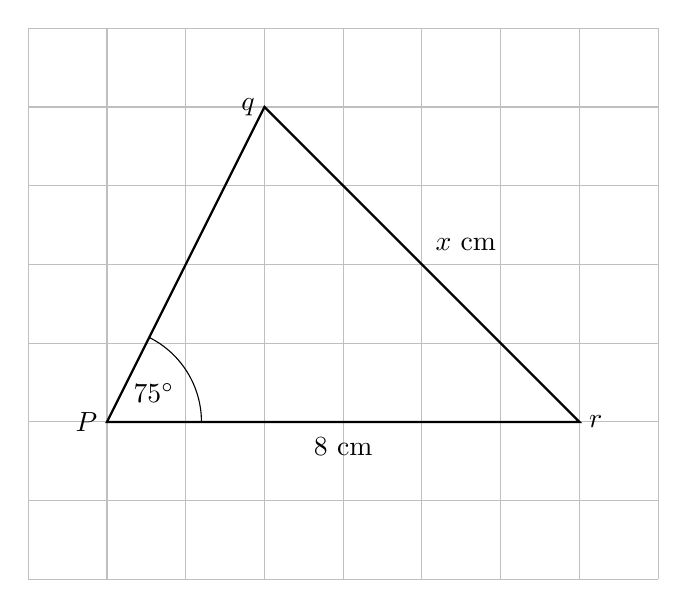
\begin{tikzpicture}




\draw[lightgray](-1,-2) grid (7,5);


\coordinate[label = left:$P$] (p) at (0,0);
\coordinate[label = left:$q$] (q) at (2,4);
\coordinate[label = right:$r$] (r) at (6,0);

\draw[thick] (p) -- (q) -- (r) -- cycle;


\tkzLabelSegment[below = 2pt](p,r){$8$ cm}
\tkzLabelSegment[above right = 2pt](q,r){$x$ cm}


\tkzMarkAngle[mark=none, size = 1.2 cm](r,p,q)    % marks the angle <rpq.
\tkzLabelAngle[pos=0.7](r,p,q){$75^{\circ}$}






\end{tikzpicture}

\end{document}




